%%This is a very basic article template.
%%There is just one section and two subsections.
%%\usepackage[utf8]{inputenc}



\documentclass{article}
\usepackage{listings}
\usepackage{graphicx}
\usepackage[pdftex]{graphicx}
\DeclareGraphicsRule{*}{mps}{*}{}

\graphicspath{ {images/} }
\begin{document}

\lstset{
  language=Java, % the language of the code
   basicstyle=\tiny                
}


\title{Testing in web/vaadin applications (plan)}
\date{December, 2014}
\author{Dmitrii Rogozin\\ Department of Pervaisive Computing, Tampere University
of Technology}
\maketitle
\abstract
Will be written at the end of the work(100-150 words)

\iffalse
	\section{Introduction (1-2 page)}
		Also probably written or massively editted at the very end.	
		\subsection{Describing the problem 1-2 paragraphs}
	    \subsection{Short summary what the paper will present 1-2 paragraphs}
	    \subsection{What data and methods you are going to use}
	    \subsection {Resutls - what are the main results of the paper}
	    \subsection {Structure of the thesis} 
	    	Section/chapter - short description
\fi
\subsection{Introduction}

		Web applications provide critical services to our society,
	 ranging from the financial and commercial sector,to the public
	 administration and health care.The wide spread use of web
	 applications as the natural interface between a service and its
	 users puts a serious demand on the quality levels that web
	 application developers are expected to deliver. At the same time,
	 web applications tend to evolve quickly, especially for what
	 concerns the presentation and interaction layer. The release
	 cycle of web applications is very short, which makes it difficult
	 to accommodate quality assurance (e.g.,testing) activities in 
	 the development process when a new release is delivered. For
	 these reasons, the possibility to increase the effectiveness and
	 efficiency of web testing has become a major need and several 
	 methodologies, tools and techniques have been developed over time.
	 
	 In these paper I will present Vaadin framework and testing tool for Vaadin,
	 called Vaadin Testbench.
	
	``Vaadin Framework is a Java web application development framework that is
	designed to make creation and maintenance of high quality web-based user interfaces easy.
	 Vaadin supports two different programming models: server-side and client-side. 
	 `` \cite[pr1.1]{bookVaaidn}
	 Vaadin TestBench is a tool for automated user interface testing of web
	 applications on all platforms and browsers. \cite{vaadinTestbenchSite}
	 
	 In the Fall 2014 I was a part of the team which developed Vaadin Testbench
	 4.0.0 and released it in the beginging of December. Web testing tools is a
	 new topic and in the this work I will represent the main ideas and challenges
	 of web testing and how they were solved during Testbench development. I will
	 also describe Vaadin framework, because Testbench is focused on testing web
	 applications written with Vaadin. I will also describe the working flow, what
	 tools and methodologies were used and how the final product might help Vaadin
	 developers.
	 
	 The goal of this work is to provide a tool for a developer, that will help to
	 write tests which can simulate user actions on the web page. The main
	 challenge is that code written with Vaadin might execute both on the
	 client-side and server-side, so that events happen on the client-side will be
	 properly sent to the server-side. Another challenge is to develop an universal
	 easy to use testing tool for Vaadin framework with a clear API.
	 
	  The result of the work was Testbench 4.0.0 released in December 2014.
	  Several user tests have shown, that a person with experience in Java and
	  Vaadin, but without any experience using Testbench, needs 15 minutes to setup
	  the envirenment and write a simple ``button-click'' test. We consider this
	  result as a success. Vaadin is an open-source project and Testbench is
	  available with free for non-comercial use license. So every person from Vaadin community can try
	  Testbench and take a look on results of our work and decide does it suits
	  his/her own needs.
	 
\section{Theoretical background}

	\subsection{Terms and Definitions}
		21st century has become an era of web applications. Software systems developed
		as a web based applcation allowes the end user to access data via web browser
		from different parts of the world and also from different devices (laptop,
		phones,tablets) has become one of the main features of modern
		applications. 
		
		Static html web sites, with little amount of javascript, which were
		constituting the big part of the Web are passing away. Modern web
		applications are very interactive and dynamic, they are becoming
		more powerful, and the difference between desktop and web applications
		dissapears. Web technologies are developing so fast, that even such domain
		specific applications as IDE(Integrated Development Dnvironment), trading
		sytems or graphic editors can be accessed via web browser. The key concept
		that helps such complicated software to become web-based is a multi-tier
		arhcitecture - the concept where the parts of the system are divided into
		separate tiers. This allows to develop presentation tier, which is
		responsible for user interface generation and lightweight validation, to
		be separate from complicated business-logic which runs on the server
		side. As a consequence the presentation tier code may be executed on different
		platforms, including web browsers. 
		
		As an extend of the growth of web applications the developing and maintaining such complicated systems becomes more and more challenging.
		All applications have a lot of common features and problems which
		were already solved by developers beforehand. This is a good practise not to
		try to reenvent a whell, but take an already made solution. That is why many
		modern applications are based on one or several software frameworks. Indeed it
		is hard to imagine that some developers team will pick a programming
		language and start to develop everything from scratch, without using any
		framework or third-party library. Same implications are applyied for testing
		frameworks. The rapidly changing and highly competitive business environment,
		choosing a right toolset is one of the key factors of the sucess. 
		
		Nowdays some companies are still rely on manual testing or ignore this
		important part of software development at all. Such approach has several
		sorrowful consequences:
		
		1. The developers are affraid of changing already written
		code. Because they do not have a confidence that their changes will break something. They
			stop cleaning their production code because they fear the changes would
			do more harm than good. ``Their production code began to rot"
			\cite[p.123]{cleanCode} 
		2. The effort of finding errors and
			fixing them raises with the amount of code written. Because the developers can not localize the place where the error is
		actual happening.
		3. Developing new features become harder,if they are based on the part of the
		system which have errors.
		
		4. All in all this leads to increasing the cost of the whole system.
	 	
	 	To test easily the huge amount code an automated web testing is come into existence.
	 	 Web testing is a kind of software testing that accentuate on web which assists to slice down price,
	  lessen the exertion requisite to check web applications as well as web sites, amplify software value,
	   condense time-to-market and reusability of test cases are also be done. 
	   
		IEEE has defined software testing as the process of evaluating a software
		system to verify that it satisfies specified requirements [3 XU]. A set of
		requirments for the web application includes security, performance,
		presentation, etc. We will focus on several requirements for the web
		application which differ from desktop application. 
		
		One of the key requirements which makes testing web applications harder than
		testing desktop applicatiosn is support of different browsers and operating systems and also
		different devices. A lot of desktop applications are developed to support some
		particular operating system or different versions of the product are developed
		and maintained for different operating systems. Web applications on the
		contrary should support not only different operating systems, but also
		different browsers and devices. So, if developers team decides to support
		three operating systems (Windows, OSX, Android), three type of devices (phone,
		tablet, PC) and three browsers (Chrome, Firefox, Internet Explorer) the number
		of possible variations is already twenty seven. If you decide to support
		different version of browsers, which in some circumstances may vary a lot,
		the number of different configurations of tested machines will be close to
		one hudred. In this case manual testing is unexceptable, because it will lead
		to unwarranted expenses. 
		
		Another difference between web and desktop applications is
		navigation on the webpage and between pages, the unexpected state change via
		the browser Back button or direct URL entry in the browser. Also some
		resources or parts of the application can be not acccessable, due to
		connection problems or maintanance. Such unexpected behaviour may happen, and
		must be handled properly, not to crash the whole application.

		Web testing includes the different type of testing like:
			- functionality tests
			- compatibility tests
			- load tests
			- performance tests
			- integration tests
		All these types of tests are equivalent important and picking a tool which
		will help to write these tests is not an easy task. It is an advantage when
		the testing tool is using same principles and similiar programming language
		with other tools in the project. We think that using same programming language
		to write both tests and code is much easier for the developer. This idea is
		related to Test-Driven Development (TDD), when tests are written
		before production code.
		
		Test-Driven Development is a very popular methodology of software
			development. The main idea is to write tests first and then code. The main
			benefits of such approach are:
				1. The developer is sure that his code works as intendent, because all his
				code is tested.
				2. The errors are found at early stage of the development cycle, which
				reduces the cost of fixing problems.
			
			Three laws of TDD \cite[pp122]{Cleancode}[Book page 122]
				1. You may not write production code until you have written a failing unit
				test.
				2. You may not write more of a unit test than is sufficient to fail.
				3. You may not write more production code than is sufficient to pass the
				curently failing test.
			\iffalse	
					\subsection {Approaches in Web Testing}	
						\begin{textit}
							In this chapter I will explain
							what does testing actually meands. What types of testing exist: unit, integration, user-interface, regression,
						etc. What are the differences between these types of testing.
						
						Next I will prove why testing is so important in software development. Here I
						would like to mention some information about \textit{Quality control}. The
						idea is to show that testing increseases the speed of software development
						and also improves it's quality. So in terms of quality control testing will
						decrease the price and increase the value of the product for the end user.
						
						Also I want to mention other methodologies like \textit{Agile development},
						\textit{User experience design} and \textit{Test Driven Development}. And how
						testing can be used/integrated with these methodologies/processes.
						\end{textit}
			\fi
	\subsection {Vaadin}	
	 ``Vaadin Framework is a Java web application development framework that is
	designed to make creation and maintenance of high quality web-based user interfaces easy.
	 Vaadin supports two different programming models: server-side and client-side. 
	 `` \cite[pr1.1]{bookVaaidn}
	 \emph{Client-side} Vaadin code is executed in the web browser as JavaScript
	 code.
	 \emph{Server-side} code is executed on the server as Java code on the Java
	 Virtual machine(JVM).
	 
	 Client-side code is originally written in Java and then
	 compiled to JavaScript using \emph{Vaadin Client Compiler}. Vaadin Client Compiler is based on Google
	 Web Toolkt(GWT) which provides the opportunity to write code in Java and
	 execute it in the browser. The client-side code is responsible for rendering
	 the user interface and send user interaction to the server.
	
	 Nowdays there are a lot of standarts and recommendations for web
	 developers published by World Wide Web Consortium (W3C) or  International
	 Organization for Standardization (ISO), including recommendations for
	 markup languages (HTML,XML,SVG), Document Object Models and standarts
	 for JavaScript. Inspite of all the standarts the difference between browsers
	 and versions might be significant for the developer. The differences may vary
	 from supporting/not supporting different CSS tags and HTML5 features,
	 different event handling and simply bugs. Vaadin client Compiler and GWT provide a wide browser
	 support, eliminating the difference between browsers, and helping a
	 developer to concentrate on essential parts of the application, instead of
	 wasting time on cross-browser support. Vaadin uses screenshot comparesment
	 (which is mentioned in part ?) as a part of regression testing, which brings
	 confindence to the developer that Vaadin components will not change their
	 appearence unexpedly with changing the version of Vaadin. 
	 
	 A server-side code runs as a servlet in a Java web server, serving HTTP
	 requests.
	 The VaadinServlet is normally used as the servlet class. The servlet receives client requests
	 and inteprets them as events for a particular user session.
	 Events are associated with user interface components and delivered to the event listeners defined in the application.
	 If the UI logic makes changes to the server-side user interface components, 
	 the servlet renders them in the web browser by generating a response.
	 
	 
	 As mentioned before both client-side and server-side code in Vaadin is written
	 in Java. This positively influences the development process in the following
	 way:
	  1. The developer does not need to know several programming languages and one
	  person may be involved in the developing of both front-end and back-end. This
	  might be an important factor for small teams and speeds up the develpment
	  process.
	  2. Vaadin brings the power of Java into the web development. Due to
	  TIOBE index \cite{tiobeIndex} Java and C are the two most popular programming
	  languages since 2002. This fact allows developer to use a great amount of
	  already-made solutions such as building tools Maven \cite{maven}, Ant
	  \cite{ant}, testing tools \cite{junit}, frameworks as akka \cite{akka} and
	  other libraries like yodatime \cite{yodatime}, guava \cite{guava} for different stages of development
	  process.
	  
	\subsection {Intergrating Vaadin with other frameworks}
	  As mentioned in (link to scratch) one of the key factors for a successful
	  development process is to pick a right toolset. Integrating server-side
	  code and other Java frameworks or libraries is easy and needs the minimum
	  amount of ``glue code''. In the following section we will show how to
	  integrate Vaadin and Akka.
	   
	  \subsection {Integrating witk Akka}
	  Akka is a Java/Scala framework for writting concurrent, fault-tolerant and
	  scalable applications. The Akka framework was adopted by many organizations
	  in a big range of industries all from investment and merchant banking, retail and social media,
	   simulation, gaming and betting, automobile and traffic systems, health care,
	   data analytics and much more\cite {akkakUseCases}. Using akka with Vaadin
	   gives an opportunity to develop concurrent, high responsive web
	   applications. Using Akka provides an
	   opportunity of developing multithreaded easily-scalable backend, when
	   changes are pushed to the client-side asynchronously(not-blocking UI). 
	   We created a sample project which solves the classical Producer-Consumer
	   problem. In this particular example Prouducer is a pool of subscriptions and
	   Consumer is a service provide, which service should be granted, according to
	   business logic.
	   
	   The main idea is the following:
		 We have one service provider, which approves requests, a request in our case
		 is a subscription for some abstract service.
		 We request several subscriptions from UI, each subscription is a thread safe task. The provider can work simulteneosly
		 only with fixed amount of tasks, if the limis is exceeded the provider sends a message to a subscription,
		 that the subscription request is put into the queue and will be initiated a
		 timeout. The information about approved subscriptions is send to the UI
		 asynchronously. The idea in this example is that when the Provider is
		 overloaded and has no resources to process the request it sends the message
		 to the client, that its request was recieved and will be processed later. The
		 client recieves this information instead of just handling. So the goal to get
		 a higly responsive application is arhcieved. The complete example can be
		 downloaded here \cite{vaadinAkka}
	
	  As we see in the above example Vaadin gives an opportunity to use already
	  made Java solutions with minimum/no overhead. The server-side code is pure
	  Java and can use a third-party framework or third-party library to ease the
	  development process. For testing server-side code we can use JUnit framework
	  which already has become a standart in the Java world.
	  
	  The difficulties come when testing client side. The client side code is
	  compiled to Javascript and executed in a web-browser, that is why we can not
	  use a Junit framework to test it. The challenge is that we need to have a
	  framework which can operate on a html page raising javascript events and
	  simulating user interaction, but also send requests related to these
	  interactions to the server side. In the following chapter we will
	  present several ideas about such testing framework.	   
	\section {Approaches in Web Testing}
		There are several approaches for web testing, the choice among them depends on
		different factors such as lifecycle of the project, technologies used, the
		budget, the professional level of developers. Two main ideas are Capture and
		Replay tests (C\&R) and programmable tests.
		
		\subsection{C\&R}
			C\&R web testing is based on capture/replay automated
			tools. \cite{CaptureReplay7} The software tester works with the web
			application modeling user behaviour, the capture/replay tool records the
			whole session and generates the script, which can be executed later,
			repeating same actions without humans participation. These scripts are then
			might be edited for comparing expected and actual resutls of the user
			actions.Script editing might be useful to adjust failed sciprts accordingly
			to the changes of the web page. Thought if the web page was changed
			significantly, editing test script might be more expensive than recording the
			test from scratch. 
			
			We must admit that C\&R approach is very popular, there are plenty of
			frameworks both for desktop and web applications such as TPTP GUI Recorder, SWTBot, QF-Test,
			Selenium IDE.
			The main advantage of this method of testing, is that the tester doesn't
			require to have experience in coding and building test cases with such tools is a simple task. 
			
			On the contrary, maintaing tests is harder and more expensive.
			The main problem is that editing generated scripts is harder than editing
			scripts written by a software debeloper. The test cases are strongly coupled
			with web pages, contain hard-coded values. These factors leads to the
			problem, that very often the tester have to record a new test, instead of
			changing the existing ones. When using C\&R tools the tester/developer can
			not use loose-coupling and decomposition, and other design tehniques to make
			easy read and maintained tests. It is hard to use parts of already made test
			cases when creating new ones if they have common parts. Basically the main
			approach is to spend a lot of time recording tests all over again and again.
			Programmable tests can help to solve these problems.
			
		\subsection{Programmable tests} 
			Programmable tests are created by a tester manually. This method requires the
			person to have programming skills and takes more time, but programmable tests
			are more flexible and allow the developer to use bigger set of tools. The
			developer may use conditional statements (to change execution of the test),
			loops (to repeat same actions), exception handling, data structures (arrays,
			sets, trees, graphs), logging, etc. Programmable tests are more flexible and
			powerful than C\&R tehnique and provides the ability to create parameterized
			tests - tests which can be executed multiple times with different arguments.
			To show that programmable tests are more powerful than C\&R we provide an
			example.
			
			Suppose we have a web framework with set of UI element classes and want to
			test that changing elements value triggers a value change listener event.
			First we create a web page where we add elements we
			want to test (textfield, combobox, radio button, etc.) and an assertion input
			element. The assertion element will include a string, which will be
			compared with expected value.
			UI elements are added to a hash map as keys.
			Strings which will be set to the assertion element are added as values to the same map. Then we
			iterate through all values in the map and add elements to the webpage and set
			their ids. We also add value change listeners, which will set
			the value of the extra element according to the event triggered. Finally we
			get a web page with set of elements. When setting value of an element with
			some id will set the assertion element to have the same id as value. For
			example if an element with an id ``textfield'' changed its value the
			assertion element will have string ``textfield'' as value.
					
			\begin{lstlisting}
			 public class TestWebPageClass {
			   static final String ASSERT_ELEM_ID="assertElementId";
			   static Map<AbstractElement,String> map = new HashMap();
			   static  {
  			   map.put(new TextField(),"textField");
  			   map.put(new ComboBox(), "combobox");
			   }
			   
			   TextField assertionElement=new TextField();
			   public void createTestWebPage () {
			    Iterator it = classToAssertValue.entrySet().iterator();
			    while (it.hasNext()) {
			     it.getKey().setId(it.getValue());
			     addElementToWebPage(it.getKey());
			     it.getKey().setValueChangeListener(event-> {
			       assertionElement.setValue(it.getValue());
			     });
			    }
			    addAssertElement();
			   }  
			   public static <AbstractElement,String> getMap() {
			     return map;
			   }
			 }
			\end{lstlisting}
      
      In our test we iterate through all elements in the map and find the
      element on the test web page by id. Then set a value to this element,
      at this point the value change listener of the element should be triggered and set the value
      of the assertion element. In the last step we compare the value in the
      assertion element with a value in the map.
			
      \begin{lstlisting}
      public class ValueChangeListenerTestClass {
       <AbstractElement,String> map=TestWebPageClass.getMap();
       String assertElementId=TestWebPageClass.ASSERT_ELEM_ID;
       UIElement assertElement=findElementById(assertElementId);
       
        @Test
        public void testValueChangeListener() {
          openWebPage();
          Iterator it = map.entrySet().iterator();
          
          while (it.hasNext()) {
            Map.Entry pair = (Map.Entry)it.next();
            UIElement elem=findElementById(map.getValue());
            elem.setValue(``foo'');
            String assertMessage=``Element with id=''+pair.getValue()
            + ``has wrong value'';
          
          Assert.assertEquals(assertMessage,assertElement.getValue(),
          pair.getValue);
          }
       }
      }
			\end{lstlisting}
  
      As mentioned before, the biggest advantage of programmable tests against
      C\&R is scalability. When using programmable tests, testing new elements
      requires just adding these elements to the map. But when using C\&R a
      tester should record same actions for each new element. If later for
      example we decide to have a test that checks that getValue() mehtod
      returns the same value as it was set with setValue method we can create
      a new test method which will use the same map of elements. 
      \begin{lstlisting}
        //test getValue() and setValue()
        @Test
        public void testSetValue() {
          openWebPage();
          private String testValue="foo";
          Iterator it = map.entrySet().iterator();
          while (it.hasNext()) {
             Map.Entry pair = (Map.Entry)it.next();
            UIElement elem=findElementById(map.getValue());
             elem.setValue(``foo'');  
             Assert.assertEquals(elem.getValue(),testValue);        
          }
        }
      \end{lstlisting}

      As a result we can see that thought writing programmable tests with
      compare to C\&R is harder and requires more experience and skills, they
      provide more flexibility and scalability. The empirical study
       of developing tests for four different frameworks shows that the development of programmable tests is more time
      consuming (between 32\% and 112\%), but test maintanance requires less
      time (with a saving of 16\% and 51\%). As a result ``In general, programmable test cases are more
expensive to write but easier to evolve than C\&R ones, with an advantage after
2 releases (in the median case)''.\cite{CaptureReplay7}
\iffalse  
	\subsection{User interface testing}	
		Some information why user interface testing is important and also why
		automated user interface testing is even more important. So we are narrowing
		the scope of the problem, not to talk about all types of testing.

		
		Afterwards I will introduce Vaadin, what's the main idea behind the framework.
		Also here I will introduce Testbench tool and Selenium- the basis of
		testbench. Thought the testbench is already exists, I would like here to tell
		what are the reasons of having Testbench, why it is needed why it was started.
		What are pros and cons. Here I'm not talking in detail about Testbench, I'm
		just introducing it.
\fi
   \subsection {Other frameworks ideas}
   		Paper \cite{Xu1} and \cite{Zhongen2} describe of the capture-replay
   		tehnique.
   		The testing monitor agent chooses the user scenario (which is written by the tester/developer),
   		 then testing agent executes the scenario and outputs the testing
   		 resutls to the monitor agent. Then the monitor compares the test output
   		 with the expected result and prints the final report. The example of the
   		 test case in paper \cite{Zhongen2}
   		 \begin{verbatim}
			 <request url = “http://mytestwebsite/login.asp”> 
			 	<parameter name = “name” value = “computer”/> 
			 	<parameter name = “password” value = “hello”/> 
			</request> 
			<response> 
			 	<match op = “contains” regexp=false select = 
			 	“/html/body” value = “Login Error!”/> 
			</response> 
   		 \end{verbatim}	
		This approach has one major disadvantage, such test framework can not test
		the application UI, it tests only server side logic, while client
		side stays untested. Another minor issue is that developer wants to write
		code and tests using same language, the reason is that code and tests are
		written in parallel, so testing framework should be very close to the
		developing framework and/or programming language.
		
		The paper \cite{testGen3} describes an improved tool for web application testing. 
			``The test driver for testing the client-side pages has the structure as
			shown in Fig.1. (1)  is the parameter initialization part. This part reads the test data and 
		 initializes parameters shown in the  user interface form. (2) is the test 
		 execution part that executes the  user interface form on the target 
		 page. In the part (2), the control  script written in the script 
		 languages like Javascript simulates event user actions in the web browser. (3) is the inner frame 
		 that contains the target page.'''
		  This tool allows to test client-side code, because the test driver
		  contains the target page and script to simulate user actions in the
		  web browser. 
		  				Figure 1
		Both approaches 1 and 2 have one major disadvantage:
			Client side testing is not complete. Thought approach includes client side
			page, it does not provide any tool for testing appearence of the webpage. The
			client side page may have bugs in css or html, for example if all html
			elements had css rule display:none, they would not be shown for user in the
			web browser. Thought all user actions could be still emulated by javascript.
	\subsection {Challenges}
		Papers \cite{Xu1} \cite{Zhongen2} and \cite{testGen3} include very simple examples
		(login page). Real-life example may have dozens/hundreds of html elements on the webpage. This is a typical
		situations in web applications, for example gmail, ebay. Navigating in big and
		branched DOM structure is not trivial. 
		There are several Methods for Locating Web page Elements:
			1. By id -locates the web page elements using their id values.
			2. By name -locates the web page elements using their name.
			3. By tag - locates the web page elements using their tag.
			4. By class - locates the web page elements using their class. 
			5. By XPath - selects a web page element by navigating the HTML tree.
		XPath is the language used for locating nodes in an XML document. As HTML can
		be an implementation of XML (XHTML), users can use this language to target
		elements in the web applications.	  
   	
   	\subsection {Selenium}
      Selenium is a set of different software tools each with a different approach
       to supporting test automation. Learning all the tools will gives different options for approaching different 
       test automation problems. The entire suite of tools allows many options for locating UI
       elements and comparing expected test results against actual application behavior.
       The opportunity to execute one’s tests on multiple browser platforms is indispensable
       in web development. 
       
       Selenium is composed of multiple software tools.
       Selenium  WebDriver makes direct calls to the browser using browser’s native support for automation.
       
       Selenium IDE - is a development environment with graphical interace for
       building test scripts.
       Selenium IDE has a recording feature, which records user actions as they are performed and
       then exports them as a reusable script in one of many programming languages that can be later executed.
       
       Selenium-Grid allows the Selenium solution to scale for large test
       suites and for test suites that must be run in multiple environments. 
       Selenium Grid allows to run tests in parallel by running different tests
       at the same time on different remote machines. Distributing tests across
       multiple physical or virtual machines gives an opportunity to execute
       tests on diffrent operating systems and browsers. 
         
   \subsection {Development of Testbench}
   	
    The plan for developing Testbench4 was from two months to six weeks. This is
    a short period of time and to manage delivering a good-quality product you
    have to minimize overhead costs. We believe that a team should choose tools
    and methodology which suits its purposes. 
    Our team decided to use Scrum for managing product development and try to be agile and flexible.
    Our team consist of two developers and a product owner. And we decided to
    have two week sprints.

    \textbf{Scrum} is a management and control process that cuts through
    complexity to focus on building software that meets business needs. Management and teams are able to get their
    hands around the requirements and technologies, never let go, and deliver working software,
    incrementally and empirically. The Scrum Team consists of a Product Owner,
    the Development Team, and a Scrum Master.
    
  \textbf{Product Owner}(PO) - decides what features should the product have to
  maximally increase the satisfaction of the end user of the product and puts this features to the backlog.
  Backlog is a set of features in priority order.
  
  \textbf{Development team} - is
  a set of professionals that are working on implementing features of the product. 
  The team size should be from three to eight people. The team should work only on tasks from the backlog.
  
  \textbf{Scrum master} - a person who should help the team to increase their
  productivity by enhancing the understanding of teams strengths and weaknesses.

  The main idea of scrum is that development is done in short-time periods
  called sprints. Each spring consists of several phases:
  Sprint planning - when team decides what tasks should be done during the
  sprint .

  Main phase - when actual development is done.
  Sprint review - when team shows/demos the results to the product owner
  Retrospective - when team discuss what can be improved.


  Sprint may take from one to four weeks. The development team should decide
  what sprint length suits their needs. During sprint planning the team chooses
  which tasks will be moved from a product backlog to a sprint backlog.
  One of the restrictions is that the task in sprint backlog should be done in one sprint.
  If the team thinks that the task can not be finished in one sprint this task
  should be divided into several subtasks. 
  Having such one-sprint tasks helps the scrum team to keep track of the
  progress easily. Besides this gives an opportunity to receive feedback for each completed task at the end
  of the sprint. This helps to detect problems at the early stages, when
  the errors does not have a tremendous feedback. So even if a feature was misunderstood by the development team
  and you have to redone it completely , the team wastes time equal to the
  length of the spring at maximum. While in a classical waterfall model, a sequential design process in which
  progress is seen as flowing steadily through the phases of all development stages, 
  the error might be found much more lately, which will have a bigger negative impact.

  Another feature of Scrum is self organization of the team. The team should
  decide by itself which toolset to use. Tasks in scrum are not assigned to developers by a manager,
  but instead developers take items from the backlog by themselves.
  This approach saves time and reduces stress, because a person can pick a task,
  which he likes and understands. Developers pick tasks that they
  can finish before the end of the sprint.

  In our case we were not developing a new product, but releasing a new version.
  We didn’t find any arguments to change the tools were used in the previous release.

  \subsubsection {Tools used}
  
  \textbf{Maven}
  Maven is a java-based software project management and comprehension tool.
  Maven is based around the central concept of a build lifecycle. This means that the process for building 
  and distributing a particular project(artifact) is clearly defined. There are three built-in lifecycles:
  default, clean and site. Users can define their own lifecycle. Lifecycles consist of phases.
   
  The default lifecycle includes the following phases:
  \begin{itemize}
    \item validate - validate the project is correct and all necessary
    information is available.
    \item compile - compile the source code of the project.
    \item test - test the compiled source code using a suitable unit testing
    framework. These tests should not require the code be packaged or deployed
    package - take the compiled code and package it in its distributable format,
    such as a JAR.
    \item integration-test - process and deploy the package if necessary into an
    environment where integration tests can be run verify - run any checks to
    verify the package is valid and meets quality criteria
    \item install - install the package into the local repository, for use as a
      dependency in other projects locally.
    \item  deploy - done in an integration or
    release environment, copies the final package to the remote repository for
    sharing with other developers and projects.
  \end{itemize}
  
  The lifecycle phases are executed sequentially, in the example above if running maven deploy 
  all the phases will be executed. All maven configurations are specified in the Project Object Model (POM) file.
  POM is an XML file that contains information about the project and configuration details used by Maven 
  to build the project. 

  Maven reduces the complexity of developing and maintaining big projects.
  Nowadays applications may depend on dozens of third-party libraries and
  frameworks. Managing those dependencies manually is very time consuming. You
  need to find and download the exact version of the library and add it to your project build path.
  The libraries might have new versions you want to use, so you need to keep track of the versions
  of the dependencies and the versions of your application, because the might be incompatible. 
  You may want to have different configurations of your application for development and production or testing.
  And all the members of your team may have same or different configurations.
  Eventually, the complexity of managing your system will grow extremely. Maven helps to solve it.

  For example to define dependencies you define a dependency section in your POM file:
  \lstset{language=XML}
    \begin{lstlisting}
      <dependency>
         <groupId>group-a</groupId>
         <artifactId>artifact-b</artifactId>
         <version>1.0</version>
      </dependency>
    \end{lstlisting}  

  Afterwards all you team members will have the same dependency downloaded and
  added to your project. If you want to have different configurations for
  development and production you can specify the profile in your POM.
   \lstset{language=XML}
    \begin{lstlisting}
      <profile>
         <id>test</id>
         <activation>
            <property>
               <name>env</name>
               <value>test</value>
            </property>
         </activation>
      </profile>
    \end{lstlisting}
  Afterwards you can pass the profile name to the maven build phase as
  a parameter.

  Eventually, you have a set of predefined configurations for your application
  for the whole team. So any developer can checkout pom file from the repository
  call mvn deploy and he will have the same version of the application with all
  the specified parameters and downloaded dependencies. If you want to update
  your dependencies or you found an error in the pom file after you fix the
  problem, all your team members have to just checkout the new version of POM.
 
  \textbf{Trac}
  Trac is an enhanced wiki and issue tracking system for software development
  projects. Trac may include several projects and users or developers can
  create tasks (also called tickets) for these projects. The tickets may have different types:
  “new feature”, “enchantment”, “error/bug”. At the beginning of the project the product owner
  goes through the list of the tickets and add them to a new milestone.
  Milestone is a plan for the next release, which includes set of tickets.

  Tickets have different value for the end user, but developers can not always
  assess that value by themselves. Product owner should help the development team to figure out the
  value of each ticket for the end user. Based on the value and time estimation each ticket should be prioritized.
  Prioritizing tickets is a very important task and should be done as soon as
  possible, preferable before coding starts. This gives a clear vision for all
  members of the team what should be done.

  In the Testbench4 project we used the trac milestone as a product backlog. On
  the sprint planning we estimate which tasks can be completed at the end of the sprint 
  and move them to the sprint backlog. As sprint backlog we used a scrum board.
  Scrum board is a white board, divided into several sections for example “to be done”, “in progress”, “in review”,
  “closed”. Paper stickers represent tickets and the person who is working on
  the ticket. The workflow is the following - a developer picks the
  ticket from the sprint backlog queue called “to be done” 
  writes his name on the sticker and move it to the “in progress” section.
  After he submitted a patch to the code review he moves the sticker to another
  section and so on.
  
  Looking to the scrum board gives you a brief summary of every team member tasks and 
  also the current sprint progress. One can also find more detailed information
  about tickets and the project progress in Trac.
 
  
  As a version control system we used \textbf{Git} - distributed revision control system
  which focuses on speed, data integrity, and support for distributed,
  non-linear workflows. There are two types of revision control systems :
  
   \begin{itemize}
   \item Client-server - such version control systems as SVN and CVS, have a 
    a centralised model, where there's a copy of the current code on a central
    server, which users check out in order to work on locally. When a user made
    some changes, he updates from the central version (in case other people have
    made changes in the meantime), solve conflicts (same part of code was
    changed by different people at the same time) that might have arisen, and
    then push their code into the server. Afterwards other people can check it out again.

   \item Distributed revision control systems such as Git, are structured on a
    peer-to-peer basis: instead of one centralised repository. Every developer
    has their own repository and there is no main repository as in client-server
    control systems, all repositories are “equal”. Though in practise developers
    create a “master” repository, where everyone push their own changes and pull
    changes made by other developers.
  \end{itemize}
  
  One of the biggest advantage of distributed systems is that repositories are
  synchronised by exchanging change-sets in the form of patches, meaning that 
  only changes are sent. In systems like SVN every time you pull changes from
  the central repository you are downloading the whole snapshot of your application sources.
  
  Also Git lets developers to have their local history of changes and commits,
  but then when pushing changes to the master repository they can rebase these changes as one commit.
  This helps on one hand keep a local history of intermediate steps for
  developer, but on the other hand have only commits for completed changes/features in the main repository
  seen for all other developers. Git has a powerful set of tools including unix commands,
  for example to find all commits made by one person you can use log command and pipeline it to a grep 
  (print lines matching a pattern) command.
  
   Git-blame command allows you to see the history of every line of your source
   code. This is very useful, if you have questions about some particular few lines of code.
   You can find an author of those lines and ask him a question.
   
   Git-bisect command - is a binary search against revision graph, which helps to find the commit which
   introduced a bug.

  \textbf{Teamcity} - is a web-based build management and continuous integration
  tool. Teamcity allows running multiple builds and tests under different platforms and environments.
  Teamcity build combines maven, ant builds, git command and bash scripts.
  
  Teamcity builds may be started automatically or manually. One option is to create a configuration to run all
  tests every night or to setup running tests on every git commit. Teamcity
  provides also build dependencies, which can be very helpful if your project
  depends on some other projects or libraries, teamcity will first build all the dependencies and then run your build.
  
  During the development cycle we used four different configurations.
  \begin{itemize}
  \item Running tests on every git commit. This configuration is started when Gerrit patch is submitted.
   Running all tests for all browsers is very time consuming and may take several hours. 
   That is why in this configuration includes only JUnit tests and PhantomJS
   tests, which does not need to run the actual browser. These kind of tests show common errors for all browsers.
   Running those tests gives a developer a fast feedback, if his changes caused some problems.
   \item Running all tests on latest commit every night. This build triggers at
    specific time every night, when servers load is lower than during the day.
    This configuration includes all the heavy tests for specific browsers. All
    the tests are run on Google Chrome, Mozilla Firefox and Internet Explorer 8, 9, 10 and 11. 
    For every test suite teamcity will run the specific browser on a test
    cluster. Running such tests is very resource consuming, but provides a
    confidence that the application is supported by all browsers.
    \item Snapshot build is run every night. This build publishes the latest
    version of the product to a maven repository.  Users can download
    the snapshot build with the latest version of the product, if they want to
    test new features, but do not want to wait for the release build.
    \item Release build is run when the team releases a new version of the
    product. This includes building all the dependencies, running all the tests,
    specifying the version of the product, creating release notes, making tag in
    the Git repository, publishing a new version to maven repository and Vaadin
    website.
   \end{itemize}

\textbf{Gerrit} is a web-based code collaboration tool. Gerrit allows developers to
  review patches made by other developers. Gerrit has a very easy system of evaluating patches:
  \begin{itemize}
  \item -2 (veto) - patch has major problems.
  \item -1 (disapprove) - patch has minor problems.
  \item +1 (approve) - no problems found.
  \item +2 (approve) - can be pushed to master.
  \end{itemize}
  
  The difference between +1 and +2 is that the patch can not be pushed to git
  repository without having +2. The reviewer can give +1 if he is not sure about his level of competence
  and want someone else to inspect the patch. There are might be several configurations of the review process,
  Figure 1 shows the process used in the Testbench4 project.

  Firstly, a developer submits his changes(patch) to Gerrit. Gerrit triggers the
  specific build in Teamcity. This build includes building the project and
  running tests. After this step is finished, teamcity returns a report about the build, if there are problems 
  the report is send to the developer and the patch is marked as -2. If all
  tests pass gerrit marks the patch as ready for review and put it to the list of waiting for review patches.
  Then the reviewer evaluates the patch. Given the patch -1 or -2 means that the developer should fix the problems,
  and submit the next version of the patch. The process continues until someone
  marks the patch as +2,  meaning in can be pushed to git master repository.
    \begin{figure}
      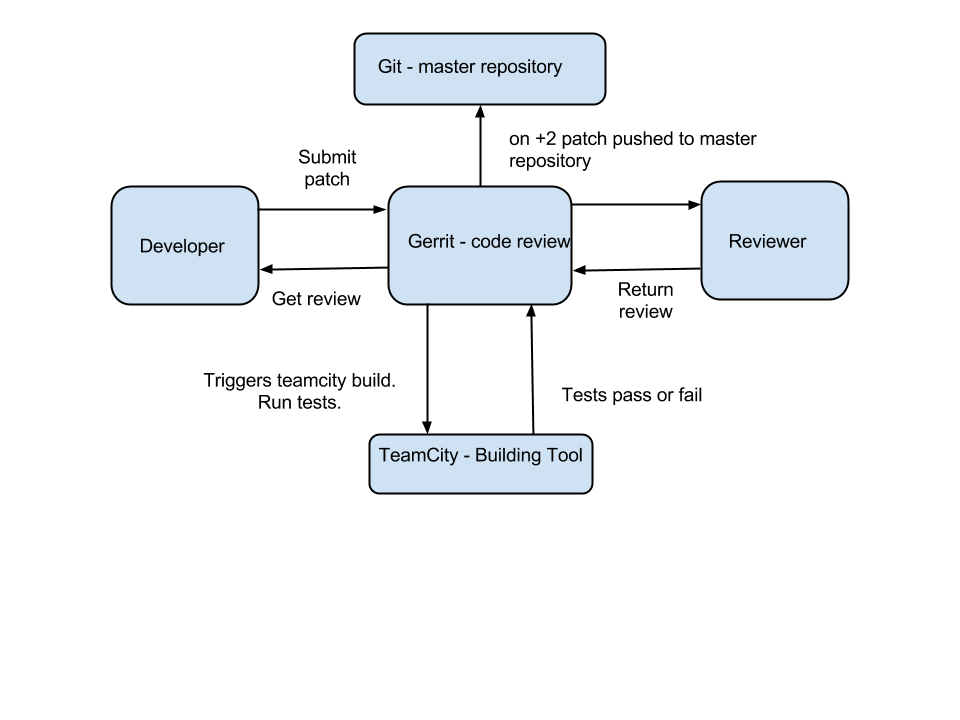
\includegraphics[width=0.75\textwidth]{gerrit1.png}
      \caption{Gerrit structure}
    \end{figure}
  Code review helps team members to follow similar code conventions, 
  keep code clean and readable and find bugs. Also code review helps developers to know more about 
  the whole project they are working in. Integrating Gerrit with an automated build tool, 
  such as TeamCity, allows to run tests before publishing commit for review. 
  The patch with failing tests is rejected automatically and an email with report for all failing tests sended 
  to the author of the patch. As an overall code review helps to keep source code quality on a higher level.


  \subsection{Testbench class diagram}
  
  \section{Example}
  \includegraphics{class.1}
  
  The hierarchy of classes in testbench consists of many tens of classes and each class has tens of methods.
  Here we will describe the most important classes and the basic principles.

AbstractHasTestBenchCommandExecutor class provides  `\$(Class<T> clazz)' and
`\$\$(Class<T> clazz)' methods which create a query for searching elements of
the given type.
 `\$' method builds a recursive search query and `\$\$' a non-recursive one.
 Non-recursive search query looks only for direct children of the element, while it’s recursive analog looks
  through all children of the element. Children elements are inner html-elements.
   For example if web-page has the following DOM(Document-Object Model). 
   Button and checkbox input elements are children elements of the div element with id id1.
  \lstset{language=HTML}
    \begin{lstlisting}
      <div id=”id1”>
        <input type="button">
        <input type ="checkbox">
      </div>
  \end{lstlisting}
  
ElementQuery<T> used for locating web elements(vaadin buttons, text fields, labels, etc.) on the web-page.
 Generic parameter T specifies the type of a searched element. 
 ElementQuery class provides methods for searching the element based on element’s id,class,
  caption or other criteria. These methods can be considered as filters in the query.
   ElementQuery uses the Builder pattern, which helps to add several filters to build a specific query and after
    the query is built execute it.

For example to find all children elements which are buttons:
  \lstset{language=Java}
    \begin{lstlisting}
    AbstractHasTestBenchCommandExecutor elem = getParentElement();
    List<Button> allButtons=elem.$(ButtonElement.class).all();
  \end{lstlisting}
  
To restrict search for buttons with caption “ok” we add a caption filter to the query.
  \lstset{language=Java}
  \begin{lstlisting}
  AbstractHasTestBenchCommandExecutor elem = getParentElement();
  List<Button> allButtons=elem.$(ButtonElement.class).caption(“ok”).all();
  \end{lstlisting}
  
TestbenchElemenet - is a base class for operating vaadin components. In includes methods to access properties common to all Vaadin elements, such as getSize(), getLocation(), getCssValue(), etc. TestbenchElement class uses Selenium WebElement class as a foundation and extend it’s functionality by using JavascriptExecutor, which allows to execute JavaScript code, and change the default element behaviour. 

ButtonElement, MenuBarElement, TableElement, etc. - implement specific class features. The default naming conventions is Vaadin component name + “Element”. In other words ButtonElement accesses buttons methods, TableElement table methods and so on. The important aspect is that hierarchy of testbench elements is similar to vaadin elements. That gives more flexibility when writing tests. Let’s look at the example:

The  developer/tester can specify concrete class for getting access to specific methods of the element:
 
 \lstset{language=Java}
  \begin{lstlisting}
  TableElement table= getElement();.$(TableElement.class).first();
  TableRowElement row=table.getRow(0);
 \end{lstlisting}
or use a more generic class to utilize method of a parent class, for example get caption of all elements :

  \lstset{language=Java}
  \begin{lstlisting}
  List<TestBenchElement> elements= getElement().$(TestBenchElement.class).all();
  List<String captions=new ArrayList<String ();
    for(int i =0;i<elements.size();i++) {
      captions.add(elements.get(i).getCaption());
    }
  }
  \end{lstlisting}

This means that actions done by user on the client side may affect the server side. Server side of the component has a state, and client-side events can change it.  Client-side of different components may look and behave exactly the same, thought
the server side behaviour is different. In practise it leads to different implementaions of same method for different components, thought the client side behaves similar. The challenge here is that we 
need to test both client and server side for each component.

Because Vaadin is a statefull framework this brings additional complexity in testing client-side and server-side communications. When event happens on the client side it will notify server side. If this event affects the server side state, the server side will notify the client side about this change. Because of a network delay or long time code execution on the server side there might be a delay between client side action and the change on a client.  In these circumstances the client-side should wait for server side code to execute, because it might affect the next client side instruction. To handle this situation Testbench has waitForVaadin method, which suspend code execution until there is no work to be done on the client side. 
      
  
    \lstset{language=Java}
    \begin{lstlisting}
      public class TestUI extends UI{
        @Override
        protected void init(VaadinRequest request) {
          createUI();
        }
        public void createUI() {
          //step 1 
          TextField field1=new TextField();
          TextField field2=new TextField2;
          field1.setCaption("field1");
          field2.setCaption("field2");
          
          //step 2
          field1.addValueChangeListener(e->{
            field2.setValue("foo");
          });
        }
      }
    \end{lstlisting}  
    
    \lstset{language=Java}
    \begin{lstlisting}
      public class TextFieldSetValueTest extends TestBenchTestCase{
        @Test
        protected void testSetValue() {
          //Step 3
          TextFieldElement field1 =
            $(TextFieldElement.class).caption("field1).first();
          TextFieldElement field2 =
            $(TextFieldElement.class).caption("field2).first();  
          field1.setValue("bar");
          //Step 4
          waitForVaadin();
          
          //Step 5
          Assert.assertEquals(field2.getValue(), "foo");           
        }
      }
    \end{lstlisting}  
     \subsection {What was actually done}
      So here I will mention what was actually done during Testbench4
      development process, there were 3 people working on the project for 2-3
      months. Part of the work was a bit routine, like implementing some basic
      API or fixing bugs, but I think I can find some topics which interesting
      and new/have academic value. I don't want to dig deep into details, like
      why you can not confirm editing the textfield by sending a 'Return' code.
      But describe more the methodology and approaches used.
      
   \subsection {Comparing Testbench with other tools}
    Here I will compare testbench to some other testing tools for example
    Selenium, what are benefits of using Testbench. The main idea is to focus
    that Vaadin is a client-server framework, so all Vaadin components have
    client and server side code, and it's important to test both. I want to show
    what problems may happen if using only Selenium and test only client side
    code, so that server side isn't tested. 
    
    Also I would like to compare how complicated is to right Selenium and
    Testbench tests. How much code is needed to test button click for example,
    or sending text to a textField.
    
    Compare speed of running tests. In Vaadin we run tests every night, and
    sometimes it takes too much time, so I would like to mention ,what are the
    problems/challenges in having a lot of tests.
    
   \subsection {Vaadin integration}
    Testbench using some features of Vaadin framework, for example searching
    elements by vaadin selectors. So I want to describe how integration with
    Vaadin is done. What are the challenges. For example what would happen when
    using different versions of Testbench with different versions of Vaadin.
    
   \subsection{Actual use of Testbench}
    Here I would describe how Testbench is used in Vaadin. How many tests are in
    Vaadin. How we run them, how failed tests are fixed what are the problems
    and benefits. What features of the Testbench are used (parallel testing
    run, searching elements on web-page by id,name,class, xpath, etc.)
    
    Then I would like to mentioned how user/developer may use Testbench, what is
    needed. Unfortunatelly it's really hard to find data to meausure the profit
    of using testging tools. It would be really nice to have a big project and
    have development with/without testing and see the end result, but I think
    it's really unlikely to happen. But may be there were some similiar studies,
    at least for other tools.
 \section {Discussion and Conclussion}
 	Middle of April/ End of April
 	\subsection {Summary}
 	  What has been done. What were the challenges how they were solved.
 	\subsection {Advantages and disadvantages}
 	\subsection {Future work}
 	
 	
	\begin{thebibliography}{7}
	
		\bibitem{Xu1}
			Lei Xu, Baowen Xu,
			"A framework for Web applications testing.",
			Proceedings of the International Conference on Cyberworlds.2004, pp.300-305
		\bibitem{Zhongen2}
		Qian Zhongsheng,Miao HuaiKou,Zeng Hongwei.
		 A practicalweb testing model for web application testing[C] .
		 Third International IEEE Conference on Signal-Image Technologies and
		 In-ternet-Based System. 2007, pp.434-441.
		 
		\bibitem{Cleancode}
		Robert C. Martin,
		Clean Code: A Handbook of Agile Software Craftsmanship,
		Prentice Hall PTR, Upper Saddle River, NJ, 2008
		
		\bibitem{testGen3}
		Seung Hak Kuk, Hyeon Soo Kim,			
		"Automatic Generation of Testing Environments for Web Applications.",
		Computer Science and Software Engineering, 2008 International Conference on
		(Volume:2 ). 12-14 Dec. 2008, :694 - 697
		
		\bibitem {selenium4}
		M. Leotta, D. Clerissi, F. Ricca, C. Spadaro,
		"Repairing Selenium Test Cases:An Industrial Case Study about Web Page
		 Element Localization," in the Proc. of Sixth International Conference on Software Testing, Verification and Validation, pp. 487-488, 2013. 
		\bibitem{pageObject5}
		M. Leotta, D. Clerissi, F. Ricca, and C. Spadaro. Improving test suites
		maintainability with the page object pattern: an industrial case study.
		In Proceedings of the 6th International Conference on Software Testing, Verification and Validation Workshops,
		ICSTW 2013, pages 108-113. IEEE, 2013. 
		\bibitem{CaptureReplay7}
		
		
		\bibitem{performance6}
		Angmo R. , Sharma M.	
		Performance evaluation of web based automation testing tools.,
		Confluence The Next Generation Information Technology Summit (Confluence),
		2014 5th International Conference. 25-26 Sept. 2014, pp. 731 - 735
		\bibitem {bookVaaidn} 
		 Author name.
		\bibitem {tiobeIndex}
		http://www.tiobe.com/index.php/content/paperinfo/tpci/index.html
		\bibitem{vaadinTestbenchSite}
		https://vaadin.com/add-ons/testbench
		\bibitem {maven}
		http://maven.apache.org
		\bibitem {ant}
		http://ant.apache.org
		\bibitem {junit}
		http://junit.org/
		\bibitem {yodatime}
		http://www.joda.org/joda-time/
		\bibitem {guava}
		https://github.com/google/guava
		\bibitem {akka}
		http://akka.io/
		\bibitem {akkaUseCases}
		http://doc.akka.io/docs/akka/snapshot/intro/use-cases.html
		\bibitem {vaadinAkka}
		https://github.com/rogozinds/VaadinWithAkka
	\end{thebibliography}
  \section {Appendix}
  
\end{document}

//TODO
{Other frameworks ideas} part give a name to all aprroaches or at least a link
add picture of the framework tool